\section{Introduction} \label{sec_intro}
In this paper, we are interested in solving the diffusion equation on a
polygonal mesh. We want to point the usefulness of using polygonal cells. Such
cell type present a big advantage over traditional cells type (triangles and
rectangles): polygonal cells allow for meshing flexibility. Boundary layer meshes 
can easily be set up, polygonal meshes can be generated from triangular meshes, 
and polygons can be included locally in existing meshes to improve mesh quality. 
Meshing tools such as MSTK \cite{mstk} and the Computational Geometry Algorithms 
Library \cite{cgal} may be employed to process polygonal meshes. For 
example, the radiation transport code PDT and the CFD codes Fluent and OpenFoam 
offer polygonal mesh and solver capabilities. The following features of polygonal
cells are noteworthy:
\begin{description}
  \item[Optimal partition of the space minimizing boundary/interior ratio]
  \item[Reduced number of unknowns:] To illustrate this, we assume
    one unknown per vertex in every cell, which is standard for discontinuous
    finite element transport discretizations that perform well in the thick
    diffusive regime. In the 2D hexagonal example of \Cref{fig_hex_vs_tri},
    the number of unknowns would be six (one unknown per vertex). Using
    triangular cells, the same hexagon would have to be split into four
    triangles at least (thus 12 unknowns) or possibly six triangles to
    preserve symmetry (thus 18 unknowns in that case). Similarly, using
    quadrilateral cells, the hexagon would be bisected into two quadrilaterals
    at least (8 unknowns), but divisions into three of four quadrilaterals are
    also possible (thus, 12 or 16 unknowns).
    \begin{figure}[H]
      \centering
      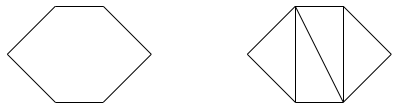
\includegraphics[width=5cm]{hex_tri_cells}
      \caption{Hexagonal cell versus triangle cells}
      \label{fig_hex_vs_tri}
    \end{figure}
  \item[Transition elements and Adaptive Mesh Refinement:] Solvers based on
    arbitrary polyhedral cells can easily handle cells with various number of
    edges. This can be particularly useful for simulations
    with Adaptive Mesh Refinement (AMR) \cite{Jessee1998,Baker2002,Wang2010a}, 
    without having to deal with the implementation of data structures to handle 
    hanging nodes \cite{Solin2008,Bangerth2007,Arnold2000}. On \Cref{fig_amr_cells}, 
    the left cell is a pentagon whereas the two cells on the right are 
    quadrilaterals. A method based on a piecewise linear discretization can
    handle locally adapted meshes without any special treatment or further
    approximation of the coupling between cells.
    \begin{figure}[H]
      \centering
      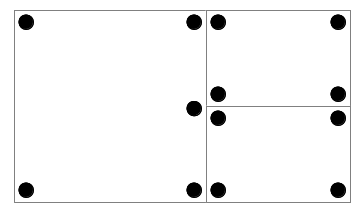
\includegraphics[width=5cm]{amr}
      \caption{AMR mesh}
      \label{fig_amr_cells}
    \end{figure}
\end{description}
Several discretization methods have been developed for arbitrary polygonal
meshes: Palmer's method \cite{Palmer2001}, mimetic finite differences
\cite{Lipnikov2004,Hyman2002,Kuznetsov2004,Brezzi2005},
Wachspress' rationale finite element \cite{Wachspress1975},
CFEM-based DFEM \cite{Warsa2008}, PWLC \cite{Bailey2008a}, PWLD 
\cite{Stone2003,Bailey2008,Bailey2008a}, and PWBLD \cite{Bailey2011}. In this
research, we focus on using PWLD to discretize the diffusion equation. The
PWLD discretization employs discontinuous finite elements and has been used to
discretize the transport equation. Using it to discretize the diffusion
equation is an important step in order to create a Diffusion Synthetic
Acceleration scheme \cite{Adams2002,Wang2010}.
In \Cref{sec_review}, we review different discretizations that can be used on
polygonal cells to discretize the diffusion equation. In \Cref{sec_ip}, we
introduce the PWLD finite elements and we use it to discretize the diffusion
equation. In \Cref{sec_amr}, we introduce the Adaptive Mesh Refinement
technique (AMR). \Cref{sec_results}, we show some numerical results. We finish
in \Cref{sec_conc} by giving our conclusions.
